\documentclass[compress]{beamer}

\usepackage[nofonts]{ctex}
\setCJKmainfont[ItalicFont={Kaiti SC}]{Kaiti SC}%
%\setCJKmainfont[ItalicFont={AR PL KaitiM GB}]{AR PL KaitiM GB}%
%\setCJKsansfont{WenQuanYi Zen Hei}% 文泉驿的黑体

\mode<beamer>
{
    \useinnertheme{rounded}
    %\useoutertheme{miniframes}
     \useoutertheme{split}
     %\usecolortheme{orchid}
     %\usecolortheme{whale}
     %\usecolortheme{lily}
     \usecolortheme{rose}
     \usecolortheme{seahorse}
}

\mode<handout>
{
	\usetheme{default}
	\usepackage{pgfpages}
	\pgfpagesuselayout{4 on 1}[a4paper,landscape,border shrink=5mm]
}


\usepackage{amsmath,latexsym,amssymb,amsfonts,amsbsy}
\usepackage{graphicx}
\usepackage{hyperref}
\usepackage{listings}
\usepackage{textpos}

\newcommand{\romannumber}[1]{{\textrm{\uppercase\expandafter{\romannumeral
#1}}}}

\graphicspath{{figure/}}

\lstset{
	basicstyle=\footnotesize, % print whole listing footnotesize
	keywordstyle=\footnotesize\color{black}\bfseries, 
	identifierstyle=\footnotesize\color{blue}, 
	commentstyle=\footnotesize\itshape, 
	stringstyle=\footnotesize\ttfamily,
	frame=single, 
	numbers=left, numberstyle=\tiny,
	stepnumber=1, numbersep=10pt,
	showtabs=false, tabsize=4,
	showstringspaces=false,
	breaklines=true, breakatwhitespace=true,
	language=[ISO]C++
}   


%%%%%%%%%%%%%%%%%%%%%%%%%%%%%%%%%%%%%%%%%%%%%%%%%%%%%%%%%%%%%%%%%
%    body                                                       %
%%%%%%%%%%%%%%%%%%%%%%%%%%%%%%%%%%%%%%%%%%%%%%%%%%%%%%%%%%%%%%%%%


\begin{document}

\AtBeginSection[]
{ 
    \begin{frame}<beamer> 
		\frametitle{内容提要} 
		\tableofcontents[currentsection,currentsubsection] 
	\end{frame} 
} 
					
\title{第一讲: Unix/Linux历史}

\author[\href{http://c.pku.edu.cn/}{http://c.pku.edu.cn/}]
{曹东刚\\\href{mailto:caodg@sei.pku.edu.cn}{caodg@sei.pku.edu.cn}}

\institute[北大信科]{Linux程序设计环境 \\
\href{http://c.pku.edu.cn/}{http://c.pku.edu.cn/}}

\date{}

\titlegraphic{
\includegraphics[height=0.17\textwidth]{Overlays/logo.pdf}}

\begin{frame}
	\titlepage
\end{frame}

\section{简介}

\subsection{初识}

\begin{frame}
\frametitle{问题}
\begin{itemize}
    \item 知道\emph{Linux}, \emph{Unix}, \emph{Posix}的区别吗?
    \item 在\emph{Unix/Linux}下编过程序吗? 
	\item 知道开源软件, \emph{GNU}吗?
	\item 能够一个学期全部使用Linux工作学习吗?
\end{itemize}
\end{frame}

\begin{frame}
\frametitle{什么是Unix}
\begin{block}{Unix 是一种多用户操作系统}
\begin{itemize}
    \item 具有悠久历史, 诞生于1969年
    \item 强大, 稳定, 高效, 昂贵
    \item 统治着高端计算市场
\end{itemize}
\end{block}
\begin{center}
 \centering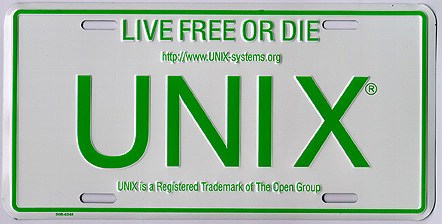
\includegraphics[scale=0.7]{unix.jpg}
 \end{center}
\end{frame}

\begin{frame}
\frametitle{什么是Linux}
\begin{block}{Linux是一种类Unix操作系统}
\begin{itemize}
    \item 诞生于1990s早期, 发展迅速 
    \item 具有Unix所有优良的特征 --- \emph{强大}
    \item 支持几乎所有的硬件 --- \emph{便宜}
    \item 开源
    \item 在服务器市场占主导, 并在桌面市场逐渐增加份额
\end{itemize}
\end{block}

\hfill
\includegraphics[height=1.0in]{Tux.png}\hfill%

\includegraphics[height=1.0in]{linux_inside.pdf}\hfill
\end{frame}

\begin{frame}
\frametitle{Unix/Linux有众多变种}
\begin{itemize}
    \item IBM AIX, SUN Solaris, SCO UnixWare, HP HP-UX, \dots
    \item Berkeley's \emph{BSD} (\emph{FreeBSD}, \emph{OpenBSD}, \emph{NetBSD}, \emph{Mac OS/X})
    \item Debian系 GNU/Linux: \emph{Debian}, \emph{Ubuntu}, \emph{Linux Mint},
        \emph{Chromium OS}
    \item RedHat系Linux: \emph{RedHat Enterprise},\emph{Fedora},
        \emph{CentOS}
    \item \emph{Gentoo}, \emph{Slackware}, \emph{Mandriva}, \emph{SUSE},
        \emph{Arch}, \ldots
    \item \emph{Android}, \emph{MeeGo}, \emph{Tizen}
\end{itemize}
\end{frame}

\subsection{特性}

\begin{frame}
\frametitle{Unix/Linux使用广泛}
\begin{itemize}
	\item Internet的心脏: WWW服务器, Email 服务器, 新闻组服务器, 应用服务器,
			数据库服务器, \dots
	\item 桌面系统
	\item 嵌入式和无线系统, 手持设备
	\item 和众多开源软件密切相关
\end{itemize}
\end{frame}

\begin{frame}
\frametitle{人们喜欢Unix/Linux}
Operating System Sucks-Rules-O-Meter\footnote{Data collected from
\href{http://srom.zgp.org/}{http://srom.zgp.org/} on Feb 17,2006}
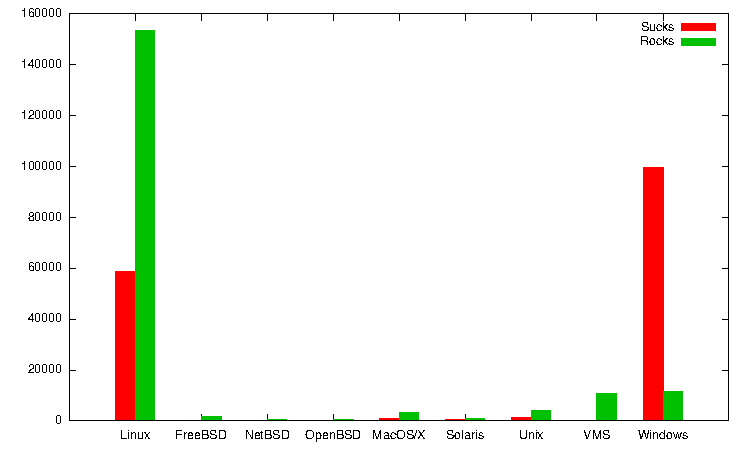
\includegraphics[width=0.8\hsize]{sucks_rocks.pdf}
\end{frame}

\begin{frame}
\frametitle{为什么喜欢Unix/Linux}

\begin{minipage}[b]{0.5\hsize}
\begin{itemize}
\item 强大健壮
\item 灵活开放
\item 开源自由(Linux)
\item 既炫且酷(Mac OS)
\item 不是\emph{M\$ Windows}
\item 以及 \pause 难以使用
\end{itemize}
\end{minipage}%
\begin{minipage}[b]{0.5\hsize}
\hfill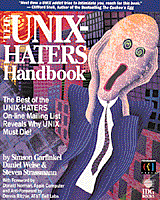
\includegraphics[width=0.5\hsize]{uhh.png}
\end{minipage}
\end{frame}

\begin{frame}
\frametitle{Case: Raspberry Pi}
\begin{itemize}
    \item 信用卡大小的全功能计算机
    \item Arm, SD卡, Raspbian Linux, Python
\end{itemize}
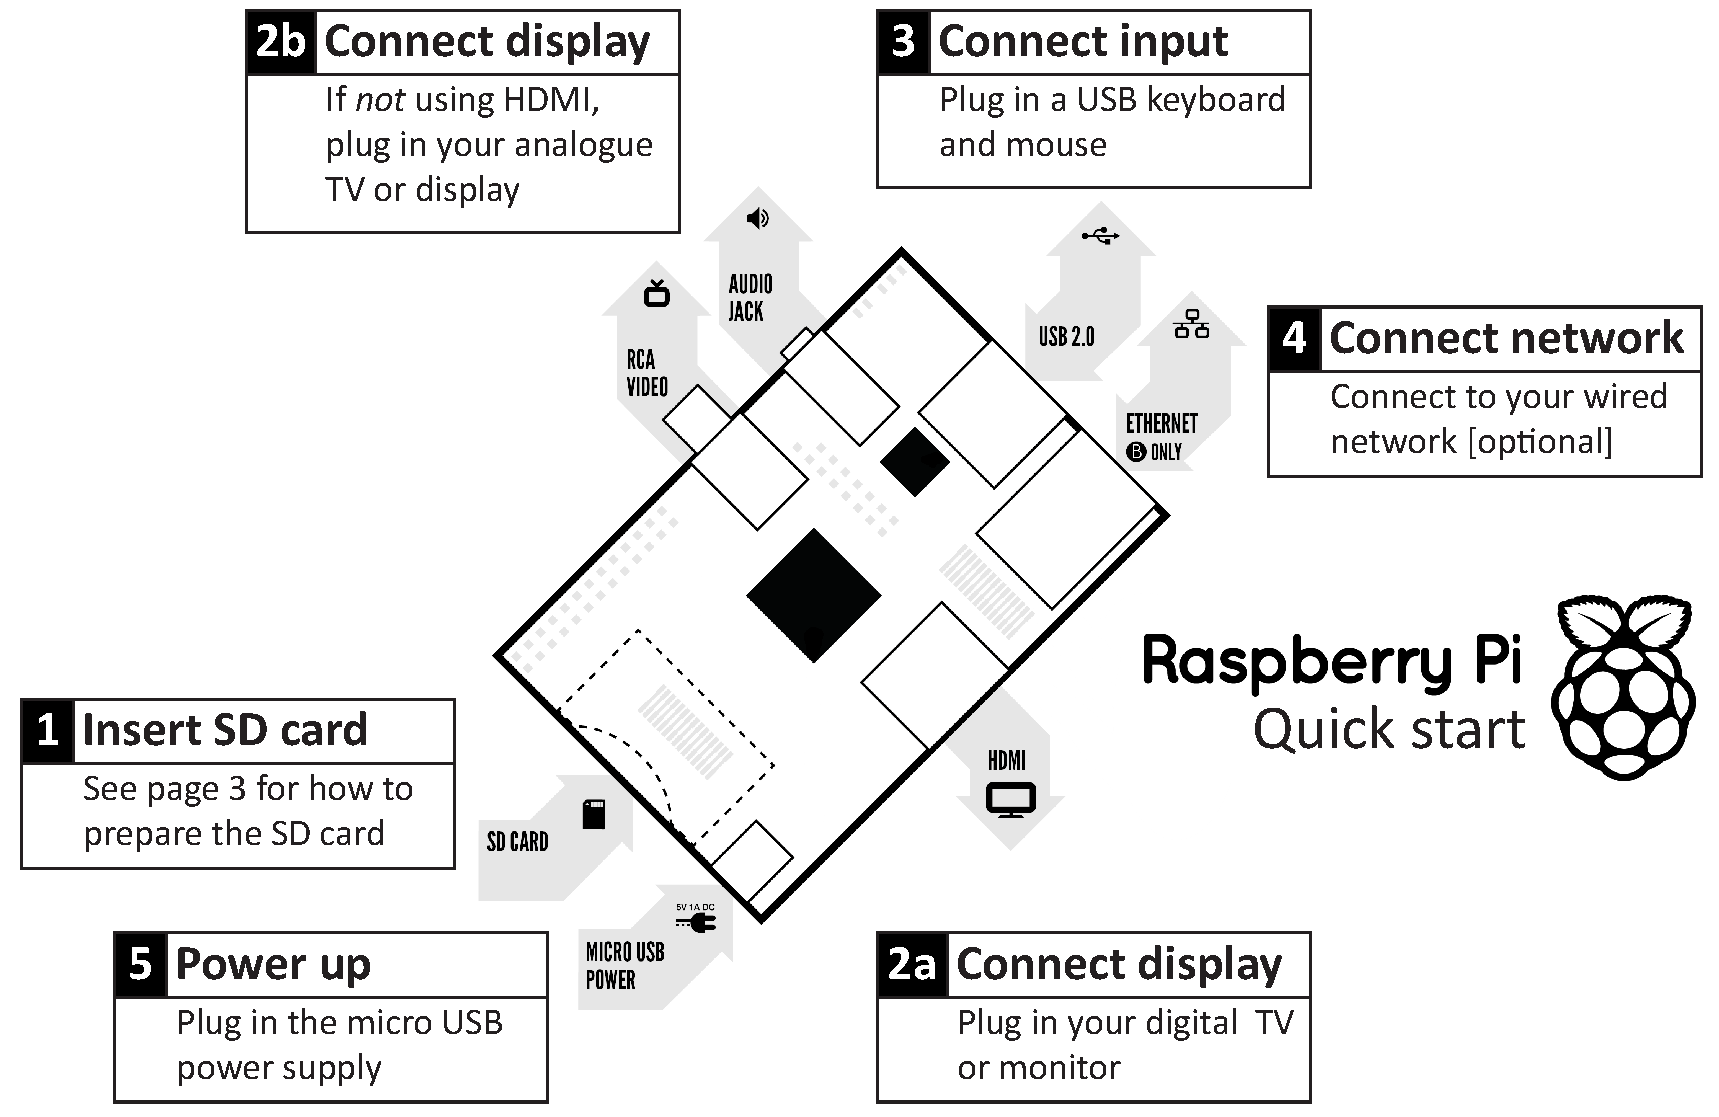
\includegraphics[width=0.8\hsize]{raspberrypi-1.pdf}
\end{frame}

\begin{frame}
\frametitle{Raspberry Pi 系统}
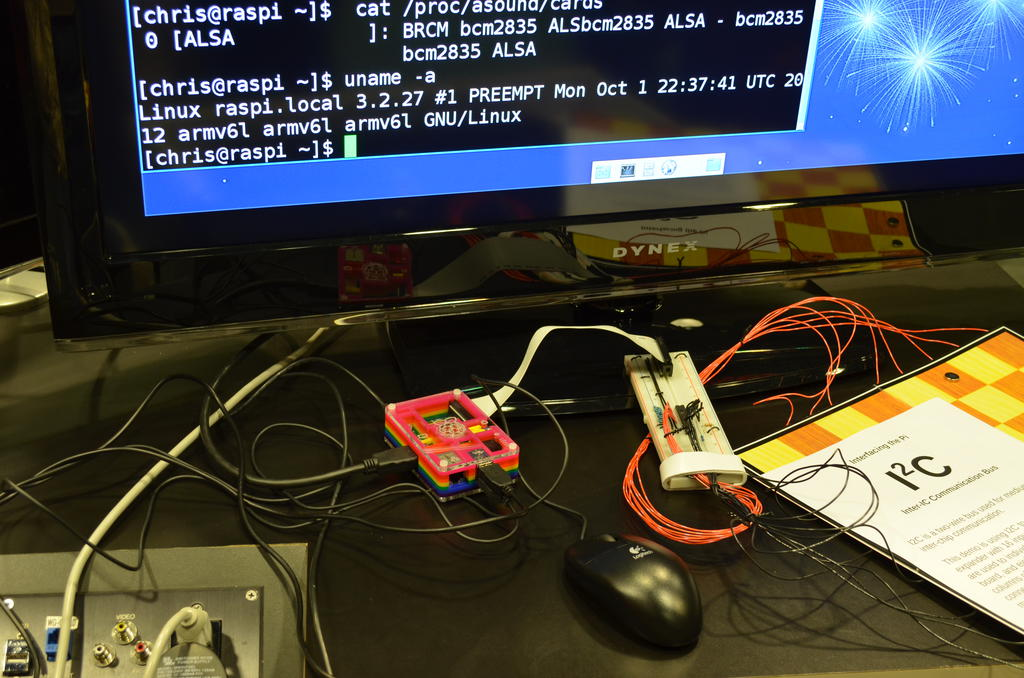
\includegraphics[width=0.9\hsize]{RaspberryPiSystem.JPG}
\end{frame}

\section{课程}

\subsection{选课}

\begin{frame}
\frametitle{谁可以选这门课}
\begin{itemize}
    \item 你已经是\emph{Unix} 用户, 但希望对Unix哲学与文化有进一步了解 
    \item 你是\emph{Linux} 新手或生手, 希望进一步提高
    \item 你是 \bfseries{计算机系学生(2年级)}!
\end{itemize}
\emph{你之所以选择它是因为需要, 而不是因为好奇!} 
\end{frame}

\begin{frame}
\frametitle{谁不应选这门课}
\begin{itemize}
    \item 希望学习详细的 \emph{C} 编程技巧
    \item 希望掌握 \emph{Unix} 内核 API(IPC, 进程控制, 套接字, 设备控制等)
    \item 希望通过计算机进行娱乐而不是工作
	\item 高年级学生
\end{itemize}
\end{frame}

\begin{frame}[t]
\frametitle{注意事项}
\alert{学习成本很高  --- 几乎所有都和\emph{M\$ Windows}不同}
\begin{block}{然而一旦入门, 收获将远远大于投入}
\begin{itemize}
    \item 无价的具有深厚积淀的经验, 哲学, 文化,
		这些将极大影响或改变你的思想与行为
    \item 很多能伴随你一生的有用工具
    \item 使你与众不同的Unix气质或偏好
\end{itemize}
\end{block}
\begin{textblock}{2}(10,0)
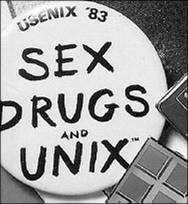
\includegraphics[height=0.8in]{unix_drug_sex.jpg}
\end{textblock}
\alert{最后, 你有可能得上Unix上瘾综合征}
\end{frame}

\subsection{上课}

\begin{frame}
\frametitle{课程内容}
\begin{itemize}
    \item 了解Unix的哲学与文化
    \item 在Unix环境中工作学习, 会使用Unix的各种工具:
    \begin{itemize}
		\item 脚本编程: \emph{sh}, \emph{awk}, \emph{sed},
            \emph{python}, \emph{perl}, \ldots
        \item 用\emph{gcc}, \emph{gdb}, \emph{patch}, \emph{make},
            \emph{autoconf}, \emph{svn}, \ldots 等工具进行程序设计
        \item 用\emph{\LaTeX}编写论文和报告
        \item \ldots
    \end{itemize}
    \item 参加开源社区, 参与甚至主导开源软件开发!
        \begin{itemize}
            \item 项目管理: 协作开发, 版本管理, 每日创建, 发布管理
            \item 基础设施管理, 服务器管理
    \end{itemize}
\end{itemize}
\end{frame}

\begin{frame}
  \frametitle{授课方式}
  课堂讲授、学生报告、项目实践
  \begin{itemize}
	\item 项目实践: 指定一个Linux开源项目贯穿整个学期的学习, 学生需要
		  \begin{itemize}
			\item 描述项目的目的和功能
			\item 进行项目分工
			\item 管理项目进度, 维护项目, 版本升级
			\item 管理项目文档, 维护项目网站
		  \end{itemize}
	\item 总结交流: 期末进行项目经验交流
  \end{itemize}
\end{frame}

\begin{frame}
    \frametitle{学生报告}
    \begin{itemize}
        \item 做过报告可以获得5分的平时成绩(满分30分)加分. 
        \item 报告应精心准备, 主要交流分享Linux使用技巧、技术分析、
            前沿技术等.
        \item 报告时间以不超过20分钟为宜.
        \item 准备做报告的同学请提前两天将报告发给教师进行申请.
    \end{itemize}
\end{frame}

\begin{frame}
  \frametitle{考核}
  \begin{itemize}
	\item 项目: 30\%
	\item 作业: 30\%
	\item 期末: 40\%
  \end{itemize}
\end{frame}

\begin{frame}
\frametitle{其他信息}
\begin{itemize}
	\item 推荐的 Linux 版本: \emph{Debian GNU/Linux}, \emph{Arch
		Linux}
\item M\$ Windows下的Linux仿真环境: \emph{Cygwin}
\item 课程主页:
\href{http://c.pku.edu.cn}{http://c.pku.edu.cn}
\item 项目孵化器: \href{http://i.pku.edu.cn}{http://i.pku.edu.cn}
\item Tel. 62757670
\end{itemize}
\end{frame}

\section{历史}

\subsection{初生 成长}

\begin{frame}
\begin{quotation}
Those who cannot remember the past are condemned to repeat it.
\begin{flushright}{\itshape The Life of Reason(1905)}\\[-0.5ex]------George Santayana\end{flushright}
\end{quotation}
\end{frame}

\begin{frame}[t]
\frametitle{诞生: 1969-1971}
The second-system effect , third-system effect

\setlength{\unitlength}{0.6cm}
\begin{picture}(13,1.5)
\put(0,0){\framebox(3,1){CTSS}} \put(5,0){\framebox(3,1){Multics}}
\put(10,0){\framebox(3,1){Unix}} \thicklines
\put(3,0.5){\vector(1,0){2}} \put(8,0.5){\vector(1,0){2}}
\end{picture}

MULTiplxed Information and Computing Service
\begin{itemize}
	\item MIT, AT\&T, GE
\end{itemize}

\begin{textblock}{4}(6,0)
\centering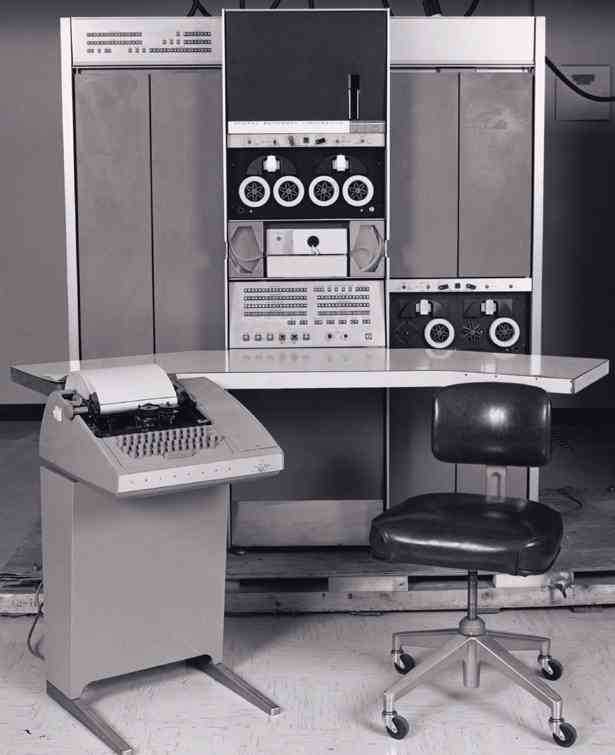
\includegraphics[width=\hsize]{Pdp7.jpg} \\
\centering{DEC PDP-7 }
\end{textblock}
\end{frame}

\begin{frame}[t]
\frametitle{Unix诞生}
Multics失败后, Ken Thompson 决定开发一个新的操作系统, 他拥有:

\begin{itemize}
\item Multics带来的灵感
\item 一台老旧的PDP-7
\item Dennis Ritchie
\end{itemize}
\emph{他只用了两天就开发成功!}
\begin{textblock}{8}(6,-5)
\centering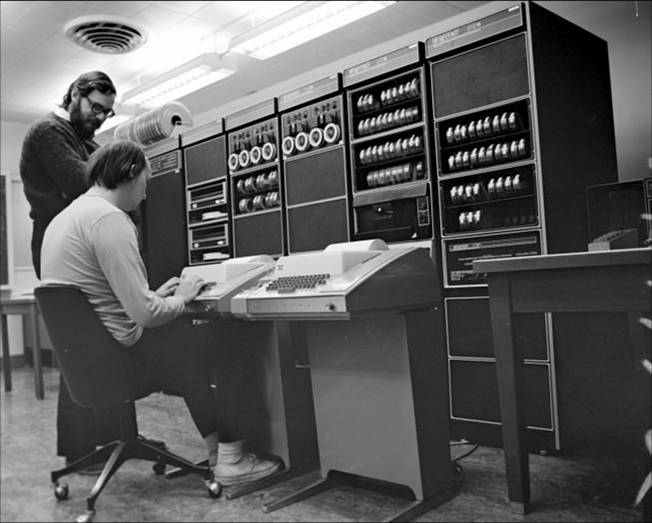
\includegraphics[width=0.8\hsize]{ken_dennis.jpg}\\
\centering{Ken Thompson 和 Dennis Ritchie}
\end{textblock}
\end{frame}

\begin{frame}
\frametitle{初生的Unix}
\begin{itemize}
\item 比同期的卡片批处理大型机系统要先进
\item 和现代Unix很相像
\item 轻量化的开发模式, 非形式化的开发方法
\item 工具: \emph{nroff}, \emph{ed}, \emph{fork()}
\end{itemize}

\begin{quotation}\fontsize{10pt}{1.0em}\selectfont
Peer pressure and simple pride in workmanship caused gobs of code
to be rewritten or discarded as better or more basic ideas
emerged. Professional rivalry and protection of turf were
practically unknow: so many good things were happening that nobody
needed to be proprietary about innovations.
\begin{flushright}{\itshape ------Doug McIlroy}\end{flushright}
\end{quotation}

\end{frame}


\begin{frame}
\frametitle{成长期: 1971--1980}
\begin{itemize}
\item 1971: Dennis发明\emph{C} 语言
\item 1973: Unix 用 \emph{C} 语言进行了重写
\item 1974: 在\textit{Communications of the ACM}发表了关于Unix的论文
\item 1975: Version 6 在 Bell Labs 之外广泛传播
\item 1976: Prof.John Lion 为 Version 6 源码增加注释
\item 1979: Version 7, 第一个现代意义的Unix版本
    \begin{itemize}
    \item \emph{C}, \emph{UUCP}, \emph{Bourne} shell
    \item 移植到\emph{VAX}机
    \item 内核超过 40 Kilobytes
    \end{itemize}
\end{itemize}
\end{frame}

\subsection{成熟 堕落}

\begin{frame}
\frametitle{TCP/IP出现 与 Unix 战争: 1980--1990}
\begin{itemize}
\item \emph{BSD} Unix 与 \emph{TCP/IP}
    \begin{itemize}
    \item 1977: Bill Joy 从 Version 6 发展出了BSD 1.x 分支
	\item \emph{vi} 出现
    \item 1983: TCP/IP 协议栈首次在 4.2 BSD 中实现--- ARPANET 和 
    Unix 两大文化开始融合
    \end{itemize}
\end{itemize}

\end{frame}

\begin{frame}
\frametitle{Unix 商业化}
  \begin{itemize}
  \item 1982: SunOS 1.0, HP-UX, Ultrix-11
  \item 1983: 针对 AT\&T 的反垄断法案
	  \begin{itemize}
	  \item \emph{System V} 商业化
	  \item 严控Unix源码分发, 高校贡献萎缩
	  \end{itemize}
  \item 1985: Intel 386 芯片发布 --- SUNs 等对此视而不见!
  \item 产品差异化造成市场分割
  \item System V 和 BSD 竞争
\end{itemize}

\end{frame}

\begin{frame}
\frametitle{困境中的进步}
\begin{itemize}
\item 1983: Larry Wall 开发了工具 \emph{\textit{patch}}
\item 1985: Richard M. Stallman 元年
    \begin{itemize}
        \item \emph{GNU} 宣言, Free Software Foundation,
        \emph{Emacs}
            \begin{itemize}
                \item \emph{GNU} : ``\emph{GNU is Not Unix}''
                \item GNU's copyleft
            \end{itemize}
        \item IEEE提出 POSIX 标准
            \begin{itemize}
            \item BSD 信号处理与作业控制, SVR3的终端控制
            \end{itemize}
    \end{itemize}
\item 1986--1987: 相继诞生了 \emph{Perl}, \emph{gcc}, \emph{X window}
\end{itemize}
\end{frame}

\begin{frame}
\frametitle{黑暗: 1989-1993}
\begin{itemize}
\item 1989--1993: Unix历史上最糟糕的时期
    \begin{itemize}
        \item Open Software Foundation: IBM, DEC, HP, \ldots
        \item Unix International: AT\&T, SUN, Intel, Motorola,
        \ldots
        \item Motorola 68000 芯片败给了 Intel 80x86 
        \item \emph{M\$} 发布了 Windows 3.0, Wintel形成
        \item GNU 未能如期开发出 free Unix kernel
    \end{itemize}
\end{itemize}
\end{frame}

\subsection{涅磐 新生}

\begin{frame}
\frametitle{曙光: 1991-1995}
\begin{itemize}
\item 1990: 1988年开始的386BSD完成, AT\&T 专用代码被从BSD Unix中清除
\item 1991: Linus Torvalds 开始了\emph{Linux} 项目
\item 1992: AT\&T 诉讼 BSDI, 使BSD失去了领先地位
\item 1991--1993: Internet 大发展, \emph{WWW} 开始流行
    \begin{itemize}
        \item 分布开发成为可能: \emph{patch}, email, newsgroups
        \item Linux 拥有 互联网, \emph{XFree86}, \emph{GNU} 工具等
    \end{itemize}
\item 1994: AT\&T 和 Novell 加入 OSF , Unix 战争结束!
\item 1995--: 开源运动新时代
\end{itemize}
\end{frame}

\begin{frame}
\frametitle{Unix 变种概览}
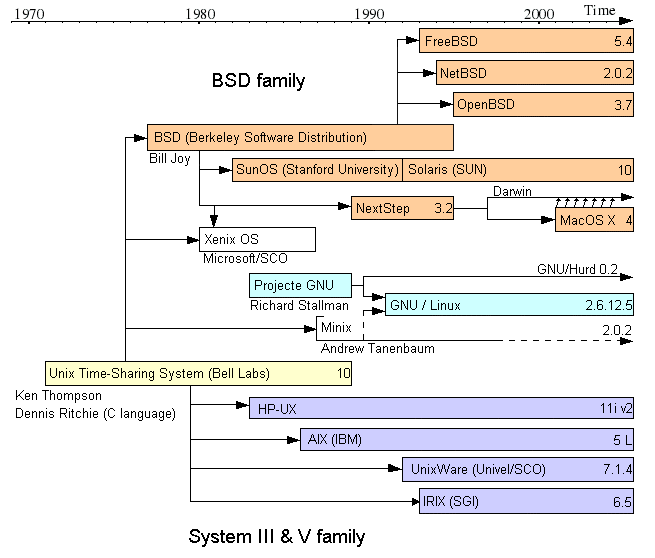
\includegraphics[width=0.8\hsize]{Unix_family.png}
\end{frame}

\subsection{黑客文化}

\begin{frame}
\frametitle{互联网与Hacker}
\begin{block}{Unix文化传统上和黑客文化相关}
\begin{itemize}
    \item 众多技术
    \item 审美观
	\item 优雅良好的设计
    \item 英雄传说
\end{itemize}
\end{block}

\end{frame}

\begin{frame}
\frametitle{学术圈: 1961--1980}
\begin{itemize}
\item Hacker 文化来源: PDP-1, MIT AI Lab, 1961
    \begin{itemize}
    \item TMRC (Tech Model Railroad Club)
    \end{itemize}
\item ARPANET 文化: PDP-10, MIT, CMU, Stanford, \ldots, 1969之后
    \begin{itemize}
    \item 负责运维 ARPANET
    \item IETF 和 RFC 的实际创建者与提议者
    \item 年轻, 聪敏, 热爱编程, 具有嬉皮士特征
    \item 并不是 Unix 程序员
    \end{itemize}
\item 网络化群体性的思维方式: ``publish or perish''
\end{itemize}
\end{frame}

\subsection{自由开源}

\begin{frame}
\frametitle{Internet出现与自由软件运动: 1981--1991}
\begin{itemize}
\item Unix 和 ARPANET 文化融合
    \begin{itemize}
        \item 始于1983, BSD支持TCP/IP
        \item 1983年, PDP-10及Jupiter项目取消, Hacker们转向Unix
        \item 完全融合, 1987
    \end{itemize}
\item Richard M. Stallman (RMS) 与 GNU
    \begin{itemize}
    \item 理念接近 Karl Marx
    \end{itemize}
\end{itemize}
\hfill
\includegraphics[height=1.5in]{gnu-head.pdf}\hfill%
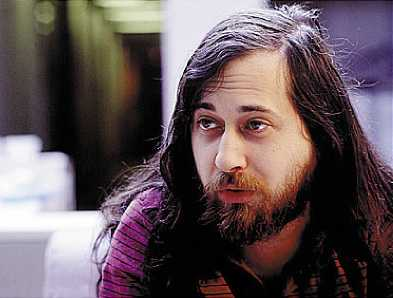
\includegraphics[height=1.0in]{Richard_Matthew_Stallman.jpg}\hfill
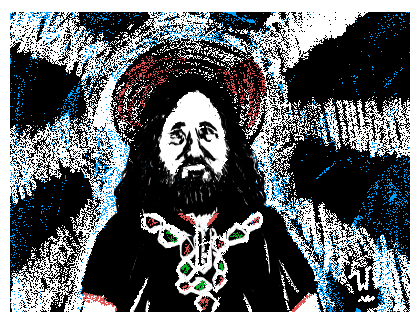
\includegraphics[height=1.0in]{Stallman.png}\hfill

\end{frame}

\begin{frame}
\frametitle{GNU 与 ``free software''}

\begin{block}{RMS的理想化政治理念}
\begin{itemize}
    \item ``free software''--- 为 Hacker们定义一种文化标签 
    \item GNU(GNU is Not Unix): 一种自由(free)的类Unix OS
	\item GPL: copyleft vs copyright
    \item GNU是一个完整的软件链, 唯独缺少一个内核---GNU Hurd
\end{itemize}
\end{block}
\begin{center}
\hfill
\includegraphics[width=0.25\hsize]{gnu-cap.jpg}\hfill%

\includegraphics[width=0.4\hsize]{gnublue.png}\hfill
\end{center}
\end{frame}

\begin{frame}
    \frametitle{其他非GNU的相近实践}
\begin{itemize}
    \item X 的开发
    \item BSD 的开发
	\item Perl,  \ldots
\end{itemize}
\end{frame}

\begin{frame}
\frametitle{Linux 和 实用主义实践 : 1991--1998}
\begin{block}{ Linus Torvalds 和 Linux 内核 }
\begin{itemize}
\item 采用 GPL license, 但并不接受 RMS 的意识形态
    \begin{itemize}
    \item 愉快的实用主义, 灵活, 低调
    \end{itemize}
\item 杀手级应用 --- \emph{Apache} 服务器 --- 1995
\item Linux 内核 + GNU 工具 $\Longrightarrow$ 一个成功 OS
\end{itemize}
\end{block}
\begin{block}{ Eric Steven Raymond 1997 年开始提出 开源 口号}
\begin{itemize}
\item 取代 RMS 敌视知识产权的意识形态
\item ``Free software
because it works better'' vs ``Free software because all software
should be free''
\end{itemize}
\end{block}
\end{frame}

\begin{frame}
\frametitle{开源运动: 1998 ~ }
\begin{block} {1998 年前的Hack群体: 松散, 各自为战}
\begin{itemize}
    \item RMS's FSF, Linux, Perl , Apache
    , BSD , X , IETF, \ldots
    \item Linux 社区展现了最大的吸引力
\end{itemize}
\end{block}

\begin{block}{ 1998 年后: 以 \emph{open-source} 为旗帜}
\begin{itemize}
\item 1998: Netscape 发布了 \emph{Mozilla} 源码
\item 1998: 开源社区领袖峰会
    \begin{itemize}
        \item 共同理念---推动 Linux 和 集市式{bazaar} 开发模型
    \end{itemize}
\item 今天: 开源理念深刻影响整个世界
\end{itemize}
\end{block}

\end{frame}

\begin{frame}
  \frametitle{今天的Linux}
\begin{block}{在争议中前行}
\begin{itemize}
\item 无尽的发行版
    \begin{itemize}
        \item Ubuntu, Fedora, SUSE, Mint, Arch, \ldots
    \end{itemize}
\item 永远的技术流
    \begin{itemize}
        \item GNOME, KDE, UNITY, XFCE
        \item Sysvinit, Upstart, Systemd
        \item XFree86, Xorg, Wayland
    \end{itemize}
\end{itemize}
\end{block}


\end{frame}

\begin{frame}
\frametitle{经验教训}
\begin{itemize}
\item When and where Unix has adhered most closely to open-source practices, it has prospered.
\item Never bet against the cheap plastic solution.
\item What the Unix community always seeks is just what it had  been doing before welcoming in all the command machinery of
business.
\end{itemize}
\end{frame}

\begin{frame}
\footnotesize
\bibliographystyle{IEEEtran}%plain, unsrt, alpha, abbrev
\bibliography{IEEEfull,reference}
\nocite{*}
\end{frame}

\end{document}
